\documentclass[twocolumn]{article}

\usepackage[utf8]{inputenc}
\usepackage{lipsum}                     % Dummytext
\usepackage{hyperref}
\usepackage{xargs}                      % Use more than one optional parameter in a new commands
\usepackage[pdftex,dvipsnames]{xcolor}  % Coloured text etc.
\usepackage{graphicx}
\usepackage{verbatim}
\usepackage{float}
\usepackage{tikz-qtree}
\usepackage{tikz}
\usepackage[linguistics]{forest}

\usepackage{amssymb}
\usepackage{amsmath}
\newcommand*{\QEDA}{\hfill\ensuremath{\blacksquare}}% filled box
\newcommand*{\QEDB}{\hfill\ensuremath{\square}}% unfilled box

% dem nice tables
\usepackage[hmargin=2cm,top=4cm,headheight=65pt,footskip=65pt]{geometry}
\usepackage{fmtcount} % for \ordinalnum
\usepackage{array,multirow}
\usepackage{tabularx}
\usepackage{lastpage}


% add a special collumn type
\newcolumntype{C}[1]{>{\centering\arraybackslash}m{#1}}


%header/footer stuff
\usepackage{fancyhdr}
\pagestyle{fancy}

%note that if you do not do these blank ones, the package defaults to something
%you may not want in your header or footer
\lhead{CMPE 293}
\chead{}
\rhead{\today}
\lfoot{Isaak Cherdak}
\cfoot{}
\rfoot{\thepage}

\renewcommand{\headrulewidth}{0pt}
\renewcommand{\footrulewidth}{0pt}

\hypersetup{
    colorlinks=true,
    linkcolor=blue,
    filecolor=magenta,
    urlcolor=cyan,
}

\usepackage[english]{babel}
\emergencystretch=1pt
\usepackage[justification=centering]{caption}
\graphicspath{{Pictures/} }

\usepackage[colorinlistoftodos,prependcaption,textsize=tiny]{todonotes}
\newcommandx{\unsure}[2][1=]{\todo[linecolor=red,backgroundcolor=red!25,bordercolor=red,#1]{#2}}
\newcommandx{\change}[2][1=]{\todo[linecolor=blue,backgroundcolor=blue!25,bordercolor=blue,#1]{#2}}
\newcommandx{\info}[2][1=]{\todo[linecolor=OliveGreen,backgroundcolor=OliveGreen!25,bordercolor=OliveGreen,#1]{#2}}
\newcommandx{\improvement}[2][1=]{\todo[linecolor=Plum,backgroundcolor=Plum!25,bordercolor=Plum,#1]{#2}}
\newcommandx{\thiswillnotshow}[2][1=]{\todo[disable,#1]{#2}}

%\usepackage{setspace}
%\doublespacing

\title{A Comparison of Persistent Data Structures for Non-Volatile Memory
Applications}
\author{Isaak Cherdak}
%\date{} %blank date

\begin{document}

\maketitle

\section*{Abstract}

With the introduction of byte-addressable persistent memory comes the need to
rethink the way that data in memory is interfaced and structured. At the heart
of this research is the consideration of various persistent data structures.
This paper seeks to determine the benefits and trade-offs of four different
persistent data structures and suggest scenarios in which each one is best
utilized.

\section*{Important terms and notations}

\begin{center}
  \begin{tabularx}{\linewidth}{ | c | X | }
    \hline
    Data structure variable & The variable in the main program referring to the
    pointer to the contents of the data structure. Most functions I standardize
    request the address of the data structure variable so that they may modify
    it if need be.\\ \hline

    PMDK & Previously known as NVML, this is Intel's library for utilization of
    persistent memory. Only libpmemobj is used in this project.\\ \hline

    Persistent & Refers to a data structure that when persisted in PMEM is
    guaranteed to be consistent and can never be in an invalid state no matter
    when a system crash occurs. \\ \hline
  \end{tabularx}
\end{center}

\section{Introduction}

Non-volatile memory (NVM) systems has become a major research focus in Computer
Science. NVM provides the possibility of byte-addressable memory that persists
across power cycles while maintaining latencies similar to that of DRAM.
Although NVM technologies have yet to reach their intended potential, there are
a number of topics of theoretical research that can be done so that NVM can be
fully utilized once it is more accessible. For example, with volatile memory,
any corruption or bugs present in memory can be cleared with a power cycle but
with NVM this is no longer an option. Thus, one requirement of structuring data
in NVM is the use of persistent data structures, or data structures whose state
cannot be invalidated. However, there are many data structures to choose from
and the potential for new ones to be created with a particular design focus.

This paper will compare four different persistent data structures in various
scenarios. First some background on major non-volatile memory system research
concerns will be discussed. Next the implementation of the data structures is
discussed including informal proof of their persistent correctness and runtime
and space utilization. Finally the paper discusses the evaluation setup and
presents results of the comparisons.

\section{Background}

\subsection{Non-Volatile Memory Based Systems}

Non-Volatile Memory Systems promise to provide memory that can survive power
cycles with the latency of DRAM\cite{burr:ibmjrd08}. However, they come with a
number of concerns such as the persistence of bugs in the kernel or applications
even after reboot.

\subsection{Software For NVM}

Byte addressable Non-volatile based memory technologies are still not
commercially available today but even so many developers are trying to create
software to maximize to potential of NVM in preparation. An example of one such
software library is Mnemosyne\cite{volos:asplos11} which among other things,
describes the concept of a shadow update. The data structures created in this
project utilize shadow updates to guarantee persistence by creating objects not
yet connected to a structure and updating pointers to the original structure in
a single operation. The result is that regardless of when a crash happens, a
data structure written in such a way cannot be invalidated.

\subsection{Analysis of Data}

Results from any test should be accurate, precise, and reproducible. The Pilot
paper\cite{li:pilot} describes this in detail. This project makes use of pilot
to determine medians in multiple trials as well as variance between tests.

\section{Implementation}

\subsection{Overview}

Four data structures exist as part of this project. The Singly Linked List,
Vector, and BTree were made by me while the LSM Tree was taken from an external
source and modified for use with this project.

Some functions listed in each data structure's documentation later in this
section are only those that I have standardized and required for each as a
critical operation used by the benchmark to generate results. Note that these
functions may have different uses or ignore some of their parameters: this is
also normal as data structures may differ in the information needed up front
during different operations (i.e: indices in BTrees). In addition, note that
insert functions assume that the entry to be inserted does not yet exist in the
data structure.

Finally, note that some of these functions are unimplemented or untested but
described for the sake of future work. Such functions will warn of this
explicitly.

\subsection{Main}

This is a C++ program which calls the Benchmark\cite{mixingc/c++}. This
originally, was intended to be used to work with libpilot and still be able to
natively call C code. In the end pilot's data analysis tool was used instead of
libpilot since libpilot took too long to get results.

\subsection{Benchmark}

This is the main program in C which directly is called from C++ Main which is
described above. The benchmark facilitates the black box tests on the data
structures. These tests are timed and are the results sent to a file for each
test. Currently there is only a basic test that performs a certain pre-specified
number of inserts and calls to get. The total amount of time for insertions and
get calls is timed and the data structure's dynamic memory usage is recorded
before destruction. The tests are also run for a number of trials to get
more accurate results from pilot's analysis tool.

\subsection{Singly Linked List}

The persistent Singly Linked List focuses on constructing nodes before
connecting them to the rest of the data structure. A list, or more specifically
the head of a list, is defined to be a pointer to a node. A sorted variant of
the list will also be described, as relevant, in each function. Note that only
the unsorted list was implemented in this project.

\subsubsection{Init}

A list of size 0, or an empty list is one where the list variable is set to
NULL. Hence, the Init function for the list simply sets the list variable to
NULL. Guaranteed persistence of this function is also trivial. Thus, the list
takes very little constant time and space to initialize.

\subsubsection{Insert}

The insert function adds a piece of data at a specified location. An item can be
added at any location that already exists or at index = size to append.
Alternatively, index = -1 means to append as well. An insert will place an item
at the specified index and "re-label" items that previously were located in the
range $[index,size-1]$ to $[index+1,size]$, hence increasing the size by 1 as
well. "Re-label"-ing of these items is simply the result of their new placement
relative to the head of the list and not a separate operation. Alternatively,
a sorted list would ignore index and place the new entry in such a way that
sorted order is maintained.

This function can also be proven persistent. Up until the point that the main
list is updated, all updates are done in the background to a single node. Hence
upon crashing, a node is either not added / leaked, or the list is successfully
updated since it takes a single pointer (either changing head or changing a next
pointer). Finally, the insert function has a worst case runtime of $O(size)$ and
space usage of $O(1)$ since iterating through the whole list may be required and
space usage will at most be that of a single node, regardless of the list's
size.

\subsubsection{Update}

This function was not implemented. The update function changes an entry in the
list whose key matches the requested key. If the entry does not yet exist, an
entry is appended or inserted in sorted order depending on whether this is an
unsorted or sorted list respectively. Updating data in a node requires the
creation of the updated node as a shadow update. Hence on crashing, the list
will either look the same as before the call to update() or will persist the
change from update(). A crash may still result in a memory leak even if the
requested update persists. Finally, since Insert is already proven to be
persistent, update is also persistent. The runtime of update is bounded above by
Insert's runtime and hence has the same asymptotic worst case runtime and space
utilization as that of Insert.

\subsubsection{Delete}

This function was not implemented. The delete function changes pointers around a
node so that the node before will change it's next pointer to the node after
this one. If it is the head, then the head is changed to point to the next node.
Since this only requires a single pointer change, this can be done without
performing shadow updates to a copied node. This function is thus persistent.
The runtime would be similar to that of insert: $O(size)$ to iterate the list to
the requested target for deletion. This function uses $O(1)$ space since it uses
the same amount of memory regardless of the size of the list.

\subsubsection{Destroy}

This function sets the list variable to point to NULL and recursively frees all
items in the list. This function is persistent but may result in memory leaks if
a crash occurs before it returns.

\subsubsection{GetElement}

This function iterates over the list and returns the item at the provided index
in an unsorted list. In a sorted list it would return the element for a key or
NULL if the key wasn't found.

\subsubsection{GetMemSize}

The return of this function is the number of bytes allocated in dynamic memory
for the data structure at the time of the call. To do this it simply determines
the number of nodes by iterating the list and multiplies by the number of bytes
taken up by a single node.

\subsection{Vector}

The vector maintains a pointer to a contiguous block of memory which doubles in
size as necessary. The vector uses an extra entry which also contains the
current capacity of the vector. This extra entry allows insertion locations to
be determined in constant time or at the very least, allows constant time
determination of whether the capacity needs to be doubled. Only the unsorted
version of this data structure was implemented but a potential sorted version is
described as well.

\subsubsection{Init}

This function allocates a contiguous block of memory with a given starting size.
The block also sets all values to an initialization value to distinguish between
an undefined and defined value. The function allocates an extra location at the
beginning of the vector which contains the vector's capacity. The vector
variable is only set to point to the block once the block is finished being
correctly constructed.

\subsubsection{Insert}

The unsorted version of this function simply adds an item at a given index to
the block pointed to by the vector. If the item is to be placed outside of the
current maximum capacity of the block, then a new block is created with a copy
of the old values and setting the rest to the uninitialized value. The vector
then is set to point to the new block and the old block is freed. Since this
function only overwrites elements in persisted blocks or changes a pointer to
another persisted block, this function is also persistent. This function runs in
worst case $O(capacity)$ time since copying a block to another block requires
iterating for the size of the block and takes $O(capacity)$ space to make another
block. If it is not necessary to double the capacity of the block then this
function takes constant time and constant space.

The sorted insert was not implemented. Sorted insert requires shifting of all
data to the right of the insertion location within the vector. To make this
persistent would be even slower since it would require a full copy into a new
vector and a final change of the vector variable.

\subsubsection{Update}

This is equivalent to insert except will overwrite the entry if one already
exists in the specified location.

\subsubsection{Delete}

This function wasn't implemented. Delete simply sets an entry to the
uninitialized value. If the index is out of the range of the current capacity
then nothing happens. Unlike insert which may double the size of the block, this
function leaves the block capacity as is. Hence, in worst case this function
runs in constant time and constant space since the location of deletion is
provided as an argument and can be checked against the capacity in constant time
by looking at the value contained in the first index.

\subsubsection{Destroy}

This sets the vector variable to NULL and frees the memory associated with the
block. This function is persistent but memory leaks may occur even if the vector
variable is set to NULL in the event of a crash.

\subsubsection{GetElement}

Returns NULL if request is out of the capacity boundary or unset and returns the
item otherwise.

\subsubsection{GetMemSize}

This function returns the amount of dynamic memory used at the time of the
function call by this data structure. In other words, it returns the size of the
block which is calculated by the capacity + 1 multiplied by sizeof a single
entry in the block.

\subsection{LSM Tree}

The implementation of an LSM Tree used in this
project\footnote{\url{https://github.com/dhanus/lsm-tree}} was created by
Harvard PhD, \href{https://dhanus.github.io/}{Deborah Hanus}. Unfortunately, the
data structure had bugs such as memory leaks and memory errors and as such
required a few fixes that I performed. I also added standardized functions to
the data structure which just call the existing functions as needed. Finally
note that this data structure hasn't been modified to be perfectly persistent.
in other words, even with persist calls, there are instances where multiple
pieces of persisted data may not be consistent with each other. Even so, calls
to persist data are used to be able to emulate the latencies of persistent
memory.

In general, an LSM Tree \cite{oneil:actainformatica96} inserts up to a certain
pre-specified number of items into memory and then into disk once memory goes
over capacity. This LSM has both an unsorted and sorted version but only the
unsorted version was used and tested here. The memory buffer was set to 256
Bytes in light of the ranges of tests used for the benchmark.

\subsubsection{Init}

This calls the LSM tree Init function which does basic initialization and
allocation of various data blocks.

\subsubsection{Insert}

If there is space in the memory buffer, insertion occurs there. Otherwise, a
merge is performed between current disk and buffer content and the merged data
is written to disk accordingly.

\subsubsection{Destroy}

This function frees the block associated with the memory buffer and clears the
file used to write data to disk.

\subsubsection{GetElement}

First checks the memory buffer for the data and then the disk. In worst case
will return NULL if not found in either.

\subsubsection{GetMemSize}

Returns the size of the dynamic memory used for the buffer block. This is
equivalent to number of entries in the memory buffer multiplied by the size of
each entry.

\subsection{BTree}

I used the original B-Tree paper\cite{comer:computingsurveys79} to get a grasp
of how I should implement this data structure. Like the list implementation, the
BTree is defined to be a pointer to a node and is NULL when empty. The BTree
operates on the rule that given an order, it has $[order,\ 2 * order]$ keys and
$[order + 1,\ 2 * order + 1]$ children per node. The keys should be thought of as
separators in the sense that values between the keys are contained in the
respective children. Finally, the above rule about minimum keys or children
doesn't apply to the root if it is a leaf. Also note this is the only data
structure that has no unsorted mode because of the nature of how it is
constructed.

\subsubsection{Init}

The BTree is initialized by being set to NULL. Hence, it has the same trivial
guaranteed persistence and runtime as the list's Init function.

\subsubsection{Insert}

The BTree's insert attempts to insert a key into a leaf node. To determine the
leaf node in question, the correct child node is iterated, based off key range.
If the leaf node is full, a complicated series of operations ensue to split
nodes from the leaf potentially all the way up to the root. These split
operations create a new node and splits left and right sides of the old node
such that each has the minimum number of keys/children and the parent receives
the median. The set of entries considered for the aforementioned split includes
the insertion entry. The functions are all carefully designed to ensure that the
data structure is persistent. This function thus has $O(log num\_entries)$ worst
case runtime and since this also reflects the maximum number of nodes to split
the space usage is $O(log num\_entries)$ as well.

\subsubsection{Update}

This function was not implemented. It only needs to replace data in a node. As a
result, we only need to copy the node, modify the value for the entry in the
copy and then have the node's parent (or the head if this is the root) change
pointers to reflect the updated node. If the data doesn't yet exist, an insert
is performed instead. Hence, the function's worst case performance is bounded
above and thus equivalent to that of insert.

\subsubsection{Delete}

This function was not implemented. an entry whose key matches the key argument
is removed. If the entry is in a non-leaf node, then you may have to perform a
recursive merge on the tree to maintain basic properties.

\subsubsection{Destroy}

This function first sets the BTree variable to NULL and then recurses into all
the current node's children. Before returning from a call to Destroy, a node
frees itself. This function runs in $O(size)$ since every entry must be freed and
in $O(constant)$ space since no additional memory is needed.

\subsubsection{GetElement}

If a key isn't found in a node, the function determines which child to search
based off key range. Returns value if key is found and NULL if the tree is
traversed without finding the key.

\subsubsection{GetMemSize}

The dynamic memory size usage of the BTree is equal to the size of all nodes in
the tree. This function recurses on the tree to get the number of nodes and
then multiplies by the size of any BTree Node.

\section{Evaluation}

The intention was to try to observe differences in performance on multiple
different machines. In the end, results were gathered from 2 different machines:
my laptop and desktop for which the specifications follow.

\begin{center}
  \begin{tabularx}{\linewidth}{ | c | X | }
    \hline
    Spec & Laptop $|$ Desktop\\ \hline \hline
    CPU & Intel core i5-6300HQ $|$ AMD Ryzen 7 1700\\ \hline
    Graphics & Nvidia GTX 960M 4GB VRAM $|$ Nvidia GTX 1060 6GB VRAM\\ \hline
    Memory & 8GB 1600 MHz DDR3L DRAM $|$ 32GB 3000 MHz DDR4 DRAM\\ \hline
    Storage & 256GB SSD $|$ 512GB SSD\\ \hline
  \end{tabularx}
\end{center}

The laptop used a persistent memory block that was 2GiB in size and the desktop
used a block that was 4GiB in size. In either case, the memory pool size was
800MB which was sufficient for tests up to 4000 inserts on all data structures
on both volatile and pmem test cases. This was done on a Ubuntu vm in both
cases.

Currently the only tests are a sequential insertion of numbers in ranges
([1,40], [1, 400], [1, 4000]) followed by a sequential set of calls to verify
that all elements can still be found inside the respective data structures.
Finally, before destroying the data structures, the dynamic memory usage is
collected.

I use gettimeofday() to collect data on runtime and a series of sizeof() calls
to determine memory usage. I used Intel's
guide\footnote{\href{https://software.intel.com/en-us/articles/how-to-emulate-persistent-memory-on-an-intel-architecture-server/}{How
to emulate persistent memory}}
on emulating persistent memory with ordinary DRAM to emulate persistent memory
performance, functionality, and primarily timings.

Furthermore, I used
clflush\footnote{\href{https://software.intel.com/sites/landingpage/IntrinsicsGuide/\#text=clflush&expand=658,657}{Clflush
from Intel intrinsics}} to flush data from the processor cache in volatile
memory tests and the
libpmemobj\footnote{\href{http://pmem.io/pmdk/libpmemobj/}{libpmemobj
documentation}} library from the
PMDK\footnote{\href{https://github.com/pmem/pmdk}{Official Intel PMDK library}}.
Finally, I used pilot to aid in analysis of the results.

\subsection{Results}

These graphs were generated using matplotlib. All the results were simply taken
from the repository just for reference. L/D refers to laptop and desktop
respectively where the number next to them refers to the number of inserts, the
number of gets after calling x inserts, and the memory size after calling x
inserts respectively.

\begin{figure}[H]
  \centering
  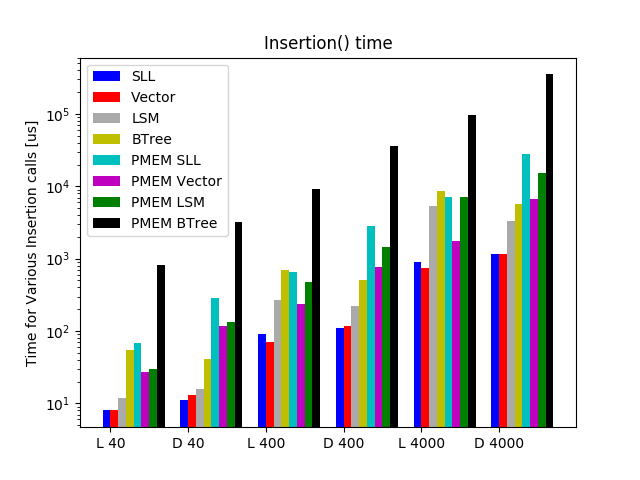
\includegraphics[width=0.5\textwidth]{insertion_times}
  \caption{The insertion times for laptop and desktop with varying insertion
  ranges. The singly linked list does really well here because all inserts are
to the head and hence constant time. Also, for some reason insertions end up
taking longer on my desktop.}
\end{figure}

\begin{figure}[H]
  \centering
  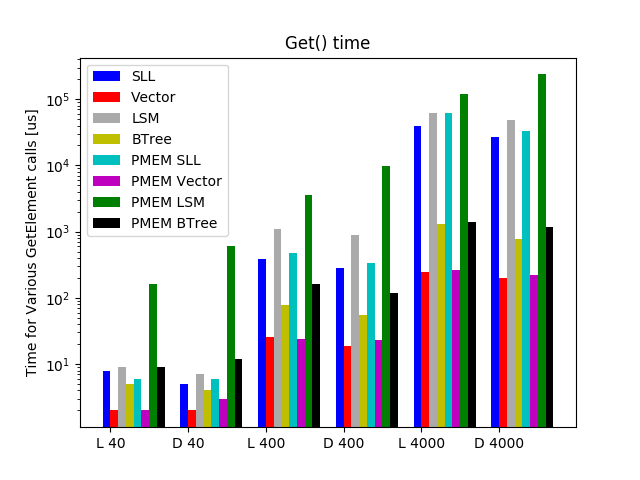
\includegraphics[width=0.5\textwidth]{get_times}
  \caption{The get times for laptop and desktop with varying insertion
  ranges. Notice in particular that this is where the BTree shines although with
only sequential tests it's not easy to see how much so. Performance between
laptop and desktop are reversed here compared to inserts where laptop
performance was better.}
\end{figure}

\begin{figure}[H]
  \centering
  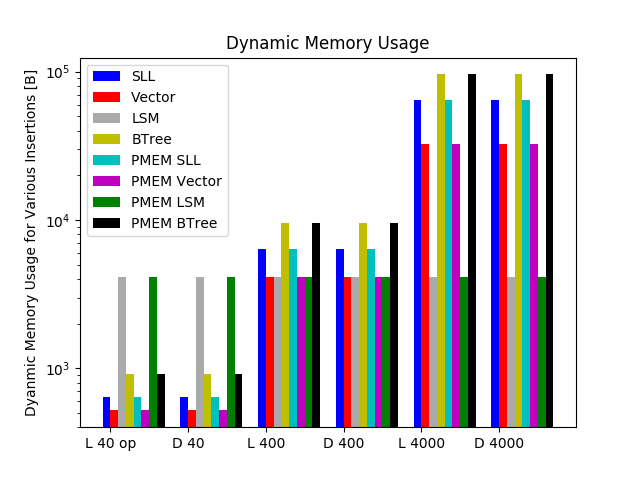
\includegraphics[width=0.5\textwidth]{memory_usage}
  \caption{The dynamic memory usage is the same on both machines as expected.
  Note that the dynamic memory usage for the LSM tree will always be the memory
buffer size which doesn't change.}
\end{figure}

\section{Major Challenges}

\subsection{Utilizing persistent memory with a familiar format}

Being able to allocate, free, and request persistence of data in a familiar
format is extremely important for code portability. However, the Persistent
Memory Development Kit (PMDK) has a lot more features and requirements than
those usually needed by a program normally using only malloc and free. As a
result, I came up with a wrapper that would allow you to call allocation or free
in a similar way. A pre-processor define allows you to simply choose whether the
program will use ordinary RAM or emulated persistent memory.

\subsection{Configuration}

Very careful consideration has to be made to ensure that everything is
configured correctly. For example, pmem test results are so much slower if you
don't correctly emulate persistent memory and don't mount onto the location used
for the persistent memory pool. Specifically, using a file location for the
memory pool not mounted on persistent memory will result in storage class
latencies (in this case flash since both computers had SSD's).

A major issue that I had been running into is the kernel code utilizing blocks
between those specified as PMEM. Such blocks will not have a device in
/dev created and as such will have no use. One way that I found gave a good
chance of receiving a functioning memory segment accessible in /dev was to split
a large segment into multiple small ones so that hopefully at least one will be
available after you reboot the new grub configuration. Another potential
solution as mentioned by the tutorial is to change the kernel configuration
which I didn't like the prospect of doing.

\section{Future Work}

A number of ideas were planned but unfortunately couldn't be integrated into the
project given time constraints.

\subsection{Improve LSM Tree}

The LSM tree would benefit from receiving testing for all components. The sorted
mode and update/delete methods would especially be useful to have tested and
ready. Most importantly, it would be nice to rewrite the data structure so it
is persistent.

\subsection{Add functionality to SLL, Vector, and BTree}

These three data structures didn't include a delete or update function. These
functions are very commonly used and it would be useful to have benchmarks on
them.

\subsection{Additional Data Structures}

Additional data structures or perhaps even variants of already existing ones
would be helpful. Some steps toward this have already been made such as the
parameter for order in the BTree which allows you to customize the minimum and
maximum keys/children per node. Note that only BTrees of order 2 were tested in
this project.

\subsection{More tests}

The project only used a simple sequential write/read test. It would be nice to
also have a random insert/read test and even tests that mix in calls to update
and delete in varying ratios. It would also be nice to have more test ranges,
especially much larger ones as it often isn't easy to characterize a data
structure's performance without a large variance in the range of tests. This was
made very clear over the course of CMPE 293.

\section{Conclusion}

The use of appropriate data structures is especially important in persistent
memory based systems. Persistent memory will likely have much worse latencies
than DRAM for a long time and major trade-offs must be made depending on the
needs of for consumers and businesses alike. At the forefront of these
trade-offs are the underlying data structures which makes benchmarking and
categorization of paramount importance. The applications of this information can
help early NVM aware software designers make better decisions about how to
structure their data.

\section{Acknowledgments}

Thank you to Ethan Miller, Daniel Bittman, and Devashish Purandere for helping
to provide ideas and helping me narrow the focus of the project appropriately.

\section{Source Code}

You can take a look at all of the source files related to the project in this
\href{https://bitbucket.org/ssrc/nvm_persistent_structures}{repository}. Note
that repository ownership is already under SSRC.

\bibliographystyle{abbrv}
\bibliography{project,bib/csrg}

\end{document}
